\section{Fundamental of Full-Bridge Converter}
A Full-Bridge Converter is a DC-DC power electronics topology designed for high-power, high-efficiency applications. It is widely used in systems requiring galvanic isolation, precise voltage regulation, and bidirectional power flow. Below is a breakdown of its core principles:
\begin{figure}[h!]
    \centering
    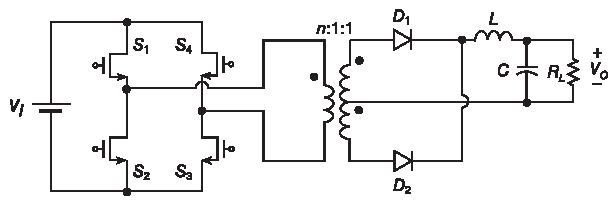
\includegraphics[width=1\linewidth]{Pictures/img/full_bridge_cir.pdf}
    \caption{\textcolor{blue}{\textit{\footnotesize Full-Bridge Converter}}}
\end{figure}
\subsection{Basic Structure}
\begin{itemize}
    \item \textbf{Four Switches:} Configured in an H-bridge arrangement (two legs with two switches each). Commonly uses MOSFETs or IGBTs for high-frequency switching.

    \item \textbf{Transformer:} A high-frequency transformer provides galvanic isolation between input and output, enabling voltage scaling via its turns ratio ($N_p : N_s$).

    \item \textbf{Rectification Stage:} The secondary side typically uses diodes (passive) or MOSFETs/IGBTs (active/synchronous rectification) to convert AC back to DC.

\end{itemize}

\subsection{Basic Working Principle}
A full-bridge converter transfers energy between input and output using four switches (\textbf{S1, S2, S3, S4}) in an H-bridge configuration. The converter alternately activates diagonal switch pairs (\textbf{S1+S3} and \textbf{S2+S4}) to generate an alternating voltage across a transformer. Below is the detailed operation:
\subsubsection{State 1: S1 and S3 ON}
\begin{itemize}
    \item Current path: \( +V_{in} \rightarrow \textbf{S1} \rightarrow \text{Transformer Primary} \rightarrow \textbf{S3} \rightarrow -V_{in} \).
    \item Applies \( +V_{in} \) across the transformer primary.
\end{itemize}
\newpage
\begin{figure}[h!]
    \centering
    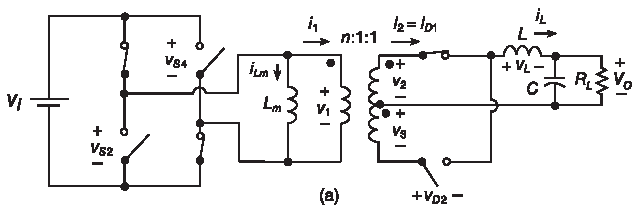
\includegraphics[width=1\linewidth]{Pictures/img/s1_and_s3_closed.pdf}
    \caption{\textcolor{blue}{\textit{\footnotesize S1 and S3 ON}}}
\end{figure}
\subsubsection{State 2: S2 and S4 ON}
\begin{itemize}
    \item Current path: \( +V_{in} \rightarrow \textbf{S4} \rightarrow \text{Transformer Primary} \rightarrow \textbf{S2} \rightarrow -V_{in} \).
     \item Applies \( -V_{in} \) across the transformer primary.
\end{itemize}
\begin{figure}[h!]
    \centering
    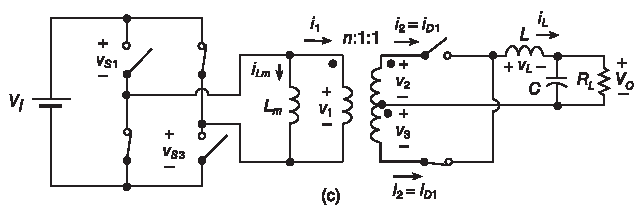
\includegraphics[width=1\linewidth]{Pictures/img/s2_and_s4_closed.pdf}
    \caption{\textcolor{blue}{\textit{\footnotesize S2 and S4 ON}}}
\end{figure}
\newpage
\subsubsection{Full-Bridge Converter CCM Waveform}
\begin{figure}[h!]
    \centering
    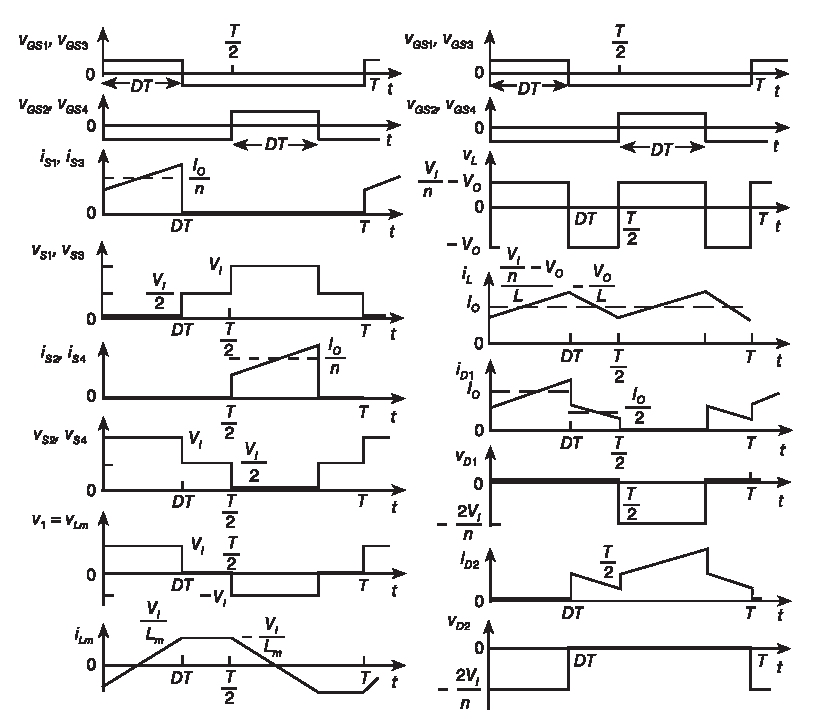
\includegraphics[width=1\linewidth]{Pictures/img/ccm_waveform.pdf}
    \caption{\textcolor{blue}{\textit{\footnotesize Waveforms of the full-bridge converter with a transformer center-tapped rectifier for CCM.}}}
\end{figure}
% \newpage
% \subsection{Basic Operation and Working Principle}
% \begin{figure}[h!]
%     \centering
%     
\includegraphics[width=0.8\linewidth]{Pictures/pics/push_pull_circuit.pdf}
%     \caption{\textcolor{blue}{\textit{\footnotesize Push-Pull Converter}}}
% \end{figure}
% \begin{figure}[h!]
%     \centering
%     
\includegraphics[width=0.8\linewidth]{Pictures/pics/duty_cycle.pdf}
%     \caption{\textcolor{blue}{\textit{\footnotesize  Switching sequence}}}
% \end{figure}
% \subsubsection*{Switch \(S_1\) ON, \(S_2\) OFF}
% \begin{itemize}
%     \item \textbf{Primary Side:}
%     \begin{itemize}
%         \item Current flows through \(S_1\) and the \textbf{first half} of the primary winding. 
%         \item The transformer core is magnetized in \textbf{one direction}.   
%         \item Primary voltage: \(V_{\text{primary}} = V_{\text{in}}\).
%     \end{itemize}
%     \item \textbf{Secondary Side:}
%     \begin{itemize}
%         \item The alternating magnetic field induces a voltage in the secondary winding.   
%         \item Rectifier diodes convert the AC voltage to DC. 
%         \item Output capacitor filters the voltage to power the load.
%     \end{itemize}
% \end{itemize} 

% \subsubsection*{Switch \(S_2\) ON, \(S_1\) OFF}
% \begin{itemize}
%     \item \textbf{Primary Side}
%     \begin{itemize}
%         \item Current flows through \(S_2\) and the \textbf{second half} of the primary winding.
%         \item Current flows through \(S_2\) and the \textbf{second half} of the primary winding.
%         \item The transformer core is magnetized in the \textbf{opposite direction}.
%         \item Primary voltage: \(V_{\text{primary}} = V_{\text{in}}\).
%     \end{itemize}
%     \item \textbf{Secondary Side}
%     \begin{itemize}
%         \item The reversed magnetic field induces an AC voltage in the secondary winding.
%         \item  Rectifier and capacitor continue delivering smooth DC to the load.
%     \end{itemize}
% \end{itemize}
% \subsubsection*{Dead Time: Both Switches OFF}
% \begin{itemize}
%     \item A brief \textbf{dead time} is inserted between switching transitions to:
%     \item Prevent \textbf{shoot-through currents} (both switches conducting simultaneously).
%     \item Allow energy from leakage inductance to dissipate via snubber circuits.
%     \item Maintain output voltage using the capacitor during transitions.
% \end{itemize}    
% \subsection{Key Components and Their Roles}
% \begin{itemize}
%     \item \textbf{Transformer}: Provides galvanic isolation and scales voltage via turns ratio (\(N_p/N_s\))
%     \item \textbf{Switches (\(S_1, S_2\))}:  Alternate between ON/OFF states to create AC in the primary (MOSFETs/IGBTs).
%     \item \textbf{Rectifier Diodes:} Convert AC voltage on the secondary to pulsating DC.
%     \item \textbf{Output Filter (L, C)}: Smooths rectified voltage to stable DC.
%     \item \textbf{PWM Controller}: Regulates duty cycle and ensures precise timing.
% \end{itemize}